
\begin{center}
\textbf{问题求解: 第一部分}	
\end{center}

计算机为什么能够帮助我们这么多? 这一部分我们来简单给出一些答案. 具体地, 我们将会了解计算思维最核心的概念,了解计算的基本方法与局限; 同时接受基本的形式化训练,掌握抽象数学证明的基本方法. 


\chapter{程序设计语言基础回顾[P]}
\begin{quote}
	心智的活动, 除了尽力产生各种简单的认识之外, 主要表现在如下三个方面:

(1) 将若干简单认识组合为一个复杂认识, 由此产生出各种复杂的认识. 

(2) 将两个认识放在一起对照, 不管它们如何简单或者复杂, 在这样做时并不将它们合而为一. 由此得到有关它们的相互关系的认识. 

(3) 将有关认识与那些在实际中和它们同在的所有其他认识隔离开, 这就是抽象, 所有具有普遍性的认识都是这样得到的. 

\hfill --John Locke 有关人类理解的随笔, 1960

\end{quote}

\section{问题的提出: 通过程序, 可以求解的问题}

电脑之所以叫“电脑”, 就是因为它能替代部分人类的思维活动. 回忆每个班上都有一个笔记和草稿纸都工工整整的Ta, 比如布置了一个很繁琐的任务, Ta总是认认真真默默画完. 很显然, 工整的笔记可以启发思维, 但是当问题范围更加大的时候非常困难继续进行. 	

学过编程的我们如果有良好的计算思维的时候, 就可能有这样的感慨: 

\begin{quote}
	烦死了! 劳资不干了! 玩更有趣的东西去了! \hfill --一名具有良好计算思维的同学
\end{quote}

这就是计算思维: 写个程序 (如model checker) 来代替我们一部分的机械的思维活动. 任何机械的思维活动都可以用计算机替代, Al还可以替代启发式/经验式的决策. 

\section{程序设计的语法与语义}

我们在学习英语的时候很重要的一部分是语法(grammar): 也就是什么样的语言是可以被接受(acceptable)的. 比如下面这个英文句子是没有语法错误的: 
\begin{verbatim}
Fuhai Zhu said that this test is only a small test, so don't panic.
\end{verbatim}
但是这句话不同人有不同的理解方式, 这就是这句话的语义(schematics). 
\begin{itemize}
\item 我们可以推断朱富海老师在安抚准备参加小测试学生们的情绪
\item 但是南京大学数学系的同学知道这是一个有名的梗: 上学期教高等代数的朱富海老师把线上期中考叫做``小测验'', 并在同学询问考试范围的时候微笑的答道:``从小学学的都考.''
\end{itemize}
\begin{quote}
简而言之(不严谨) , 现在我们有一个由一堆字符串和推导规则组成的形式系统(formal system), 语法决定了这个形式系统能生存什么样的字符串, 而至于这些字符串有什么样的含义则是语义的范畴.

语法类似材料, 语义类似与材料组成的各种建筑物, 我们可以通过语法研究语义层面的推导, 同时也可以从语义层面捕获语法中内涵的结构,
其实语法和语义是相互区别又紧密联系, 即从范畴论的角度看语法和语义是伴随的(其实不同的人做数学证明可以有不同的风格: 偏语法和偏语义,
不过大部分数学家更喜欢语义风格的证明, 可能因为更直观, 更容易被人脑接受. ) 

选自\url{https://www.zhihu.com/question/31347357/answer/892133941}
\end{quote}

\section{Python代码执行可视化: 一个网站}

\begin{tool}
在浏览器中输入\url{https://pythontutor.com/visualize.html}, 你就会得到一个Python代码执行可视化((visualization)的机器. 当对于程序执行的结果感到存在疑问的时候, 我们可以用这个网站观察Python是如何``解释''你的代码的.

比如, 下面这一小段代码: 
\begin{lstlisting}[language=python]
for i in range(10):
    print(i**2)
\end{lstlisting}

点击Visualize Execution就可以了, 你可以点击Next来继续模拟执行下一步.

在这里, 你可能会看到很多新奇的名词: 什么是Global Frame, Object? 暂时先不用管. 不过你确实可以看到点击Next的时候Print output一栏一步一步的模拟了你的代码. 
\end{tool}

通过观察可以发现, 代码按照行数执行, 一次执行一行, 每一次执行计算机内部结构的状态(右侧的面板). 下面我们化繁为简, 来看一看一个系统(数学意义上)能够完成任何人类完成的操作需要的最小可能的操作是什么. 

\begin{Exercise}\label{ex:tool1}
        以下的习题或许可以让你搞明白原来不懂的东西: 
        \Question 请找出原来让你感觉比较难以理解的小段Python代码, 放在这里来试一试, 看一看是不是更加清晰的理解了. 
        
        \Question 其实, 你可以在电脑中搭建一个这样的环境, 而不用每一次都要通过网页访问的方式做这样的事情. 具体地, 你需要配置一个调试器的环境. 那么, 这件事就拜托你去网上搜索一下吧! 

\end{Exercise}

    \begin{multicols}{2}
        \begin{Answer}[ref={ex:tool1}]
           	对于第一个问题, 可以用自己的想法去试一试.  对于第二个问题, 最好使用Google, Bing而不是Baidu进行检索. 另外, 注意接受阅读英语文献! 
        \end{Answer}
    \end{multicols}



\section{可以``程序化''执行命令的最小指令集}
如果我们说, 写出来一个可以计算``我们想要计算的任何理论上能够计算的东西''并不难, 你会不会认为这件事情是无稽之谈? 毕竟计算问题多种多样, 有一些内容涉及到很复杂的判断.  但是, 我们可以用一个很小的指令的集合来描述``我们可以计算的一切事物''. 我们不妨从日常生活中找一点灵感.
\begin{example}
(等红绿灯) 观察红绿灯, \textbf{如果(if)}是绿灯, 那就通过这个路口; \textbf{否则(else)}继续等待. (遵纪守法的好公民)

(做作业) 明确今天的作业范围, 从\textbf{第一题}开始写, 写完题目\textbf{或者(or)}一题目没有思路之后做\textbf{下一道}题,
\textbf{直到(until)}做完所有的问题.

(排序成绩单) 获得班上同学的所有\textbf{成绩单}, 拿一张新的白纸打好\textbf{表格}, \textbf{每一次(for each time)}从成绩单中选取最大的分数,
把那一行\textbf{抄写到}新的白纸上. 之后把原来那张纸上的内容划去. \textbf{一直重复下去}, \textbf{直到}原来的成绩单上没有任何可以被划去的内容.
\end{example}
我们需要找一些东西来具象化我们脑子中的``红绿灯的状态(state)'', ``现在在做作业的题目编号'', 这些内容, 因此我们就希望把这些抽象出来.
因此我们有了变量(variable)的概念, 也就是值存在的空间. 

把上面的三个内容转化成伪代码(不唯一)就是:
\begin{lstlisting}
------ GO THROUGH CONJUNCTION ------
if traffic light's color is green:
    go pass by
else
    wait

------ DO HOMEWORK ------
range = [a..b]
working on problem = a
while working on problem <= b:
    finished this problem or can't work out
    working on problem = working on problem+1

------ SORT EXAM SCORE ------
list = get the source table
result = empty(for now)
while list is not empty
    k= get the max element of list
    write k to the next line of result
show result
\end{lstlisting}
其实要是能够构造出任何程序的``原材料''(也就是我们的指令集)并不复杂. 无非就是变量(variable)的赋值(assign), 判断(judgement), 跳转(jump), 终止(terminate). 也就是, 如果你能声称有一套系统可以自动化的解决这四个内容,
那么这个系统就具有机械化地做任何人类做的事情. 换句话说, 你可以用这个工具创造整个世界. 

\begin{dialogue}
	A: 创造整个世界? 感觉好中二! 
	
	B: 有道理. 但是, 计算机的发明极大地解放了人们的计算能力, 我们只要描述更加聪明的东西, 计算机就会帮我们做更笨重的机械化的指令--而且几乎不会出错! 
	
	A: 有点意思, 毕竟我算个两位数乘两位数有时候都能出错...
	
	B: 是的, 不过这个可以交给计算机. 我们就可以专注于研究更加``高等''和``深刻''的内容了. 
\end{dialogue}

其实用``机械化''的方法代替人力这样的想法是在计算机诞生之前就是人们孜孜以求的问题. Alan Turing 在1936年就提出了这样的设想. 他就是由只一条(无限长)的纸带和一根笔(可以改纸带的内容,
并且查看纸带的内容并据此做判断), 并且有一个程序(墙上的表格), 指示下一步要往哪转移. 只要能够移动读写头, 写纸带的某一个格子,
读纸带的某一个格子, 跳转, 以及终止.  根据计算领域里的证明, 可以得到这个机器就和我们人类的计算能力等价. 

这是最早的图灵机的原型. 

\begin{figure}
\centering
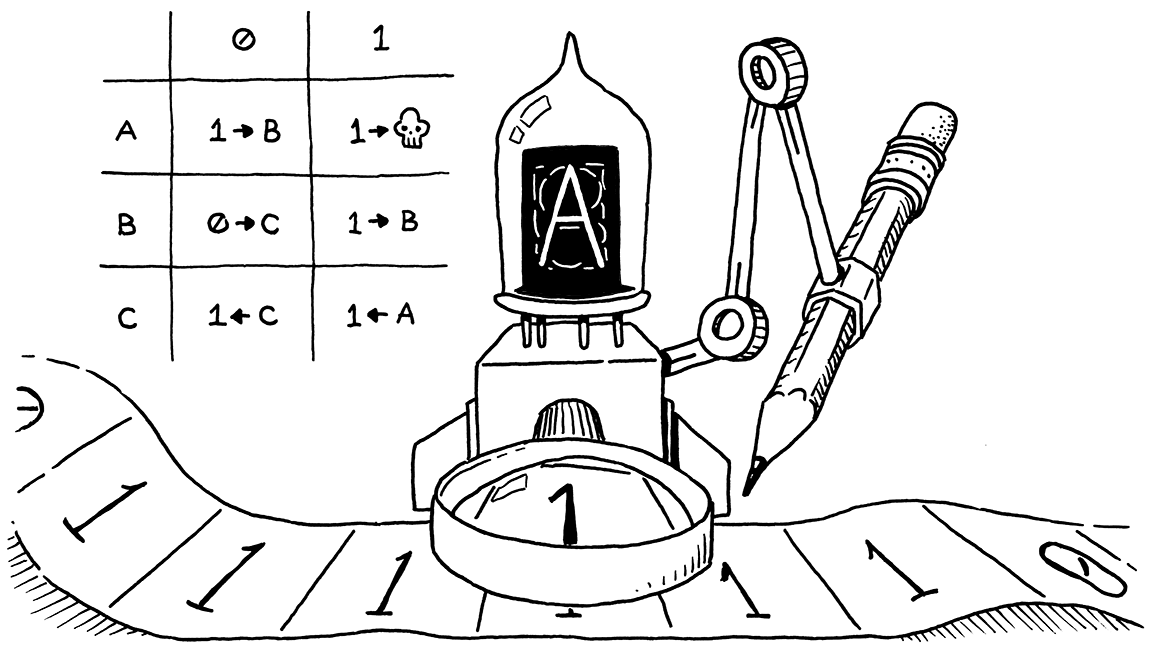
\includegraphics[scale=0.3]{1-python-plim/figs/turing-machine}	
\caption{一个存在于人类脑海中的图灵机实例}
\label{fig:trm}
\end{figure}


\begin{example}
运行图片\ref{fig:trm}的程序, 左右按照我们的左右进行(规定A\textbf{B}C右移一格是AB\textbf{C}).

(1) 现在机器的状态是A(头部的字母), 看到的是1(放大镜的字母)

(2) 于是把当前的格子改为1, 纸带向右移动一格, 然后停机.

\textbf{假设}当前纸带的放大镜看到的是0, 再运行一次:

状态:A 纸带状态: 0 1 1 1 \textbf{0} 1 1 0 0

(1)现在机器的状态是A(头部的字母), 看到的是0(放大镜的字母), 执行第一行第一列的指令$1(\text{改\text{为1)}}\rightarrow(\text{向\text{右移动一格)}}B(\text{状\text{态改为B)} . }$

状态:B 纸带状态: 0 1 1 1 1 \textbf{1} 1 0 0

(2)现在机器的状态是B(头部的字母), 看到的是1(放大镜的字母), 执行第二行第二列的指令$1(\text{改\text{为1)}}\rightarrow(\text{向\text{右移动一格)}}B(\text{状\text{态改为B)} . }$

状态:B 纸带状态: 0 1 1 1 1 1 \textbf{1} 0 0

(3)现在机器的状态是B(头部的字母), 看到的是1(放大镜的字母), 执行第二行第二列的指令$1(\text{改\text{为1)}}\rightarrow(\text{向\text{右移动一格)}}B(\text{状\text{态改为B)} . }$

状态:B 纸带状态: 0 1 1 1 1 1 1 \textbf{0 }0

(4)现在机器的状态是B(头部的字母), 看到的是0(放大镜的字母), 执行第二行第一列的指令$0(\text{改\text{为0)}}\rightarrow(\text{向\text{右移动一格)}}C(\text{状\text{态改为C)} . }$

状态:C 纸带状态: 0 1 1 1 1 1 1 0 \textbf{0}

(5)现在机器的状态是C(头部的字母), 看到的是0(放大镜的字母), 执行第三行第一列的指令$1(\text{改\text{为1)}}\leftarrow(\text{向\text{左移动一格)}}C(\text{状\text{态改为C)} . }$

状态:C 纸带状态: 0 1 1 1 1 1 1 \textbf{0} 1

(6)现在机器的状态是C(头部的字母), 看到的是0(放大镜的字母), 执行第三行第一列的指令$1(\text{改\text{为1)}}\leftarrow(\text{向\text{左移动一格)}}C(\text{状\text{态改为C)} . }$

状态:C 纸带状态: 0 1 1 1 1 1 \textbf{1} 1 1

(7)现在机器的状态是C(头部的字母), 看到的是1(放大镜的字母), 执行第三行第二列的指令$1(\text{改\text{为1)}}\leftarrow(\text{向\text{左移动一格)}}A(\text{状\text{态改为A)} . }$

状态:A 纸带状态: 0 1 1 1 1 \textbf{1} 1 1 1

(8)现在机器的状态是A(头部的字母), 看到的是1(放大镜的字母), 执行第一行第二列的指令$1(\text{改\text{为1)}}\rightarrow(\text{向\text{右边移动一格)}}\dagger(\text{停\text{机)}}$

状态:A 纸带状态: 0 1 1 1 1 1 \textbf{1} 1 1
\end{example}
下面我们来看一看为什么说可以用Python语言的计算能力和他们是等价的. 在这之前, 我们先来了解一下如何获取帮助和得到通俗易懂的教程. 

\begin{dialogue}
	A: 我最近开始学Python了. 
	
	B: 好啊, 你都学了什么?
	
	A: 我学了Python可以读作/ˈpīˌTHän/, 也可以读作/ˈpīTH(ə)n/, 是蟒蛇的意思...
	
	B: 嗯, 还有呢? 
	
	A: uhmm... 还有变量的定义是变量是存放数据值的容器. 与其他编程语言不同, Python 没有声明变量的命令. 首次为其赋值时,才会创建变量. 
	
	B: 不要背诵定义. 精确的定义毫无意义. 
	
	A: 那该怎么办? 
	
	B: 从例子中出发, 就把它当做英文说明书, 另外参考官方教程, 并且跟着官方教程做, 就会有大概的认识. 慢慢的, 你就能够得到你自己的定义了. 
\end{dialogue}

所以, 请认真阅读并实践(无论是在脑子还是在交互器(interactive shell)里面)官方帮助文档(可以在\url{https://docs.python.org/zh-cn/3/tutorial/introduction.html}找到)\footnote{最好看英文版, 更加自然一些. }的内容.
可以让你了解更多易于理解的东西. 如果文章中有描述C和Pascal的句子, 忽略它就可以. 毕竟文档是给各个不同层次和水平的人看的, 有一些看不懂以后再说. 

\begin{idea}
摒弃``我一定要一次把所有的东西都弄懂''的理念, 因为这些知识十分的巨大. 所以先了解一部分作为正确的立足点, 然后慢慢扩大就行了. 这需要很长时间的积累, 千万不要急. (着急也没用, 只会加大精神内耗.)	
\end{idea}

\subsection{Python中的整个世界}

下面的内容其实不用单独记忆, 只要明确有哪些语句, 这些语句造成的效果是什么就行了. 如果看到有任何的问题, 如果是关于英语单词的, 可以搜索字典; 如果是对于程序报错有疑问, 可以搜索文档里面关于报错的信息; 如果有其他创造性的问题, 则可以询问周围的同学和老师. 

下面会有两个术语(term), 分别是表达式(expression)和过程(procedure), 表达式可以暂且认为是形如x+12,
{[}2{]}{*}3这样的可以进行计算的内容, 过程就是一系列执行的过程, 不一定要能得到值. 我们用一个例子感受一下.


\begin{lyxcode}
def~InsertionSort(A):~~~~~~~~~~~~~~~~~~~~~~~~~~~~

~~~~for~j~in~range(1,~len(A)):~~~~~~~~~~~~~~~~~~~\#Proc

~~~~~~~~key~=~A{[}j{]}~~~~\#A{[}j{]},key~are~expr~\#Proc~~~\#|

~~~~~~~~i~=~j~-~1~~~~~\#j-1,i~are~an~expr~\#v~~~~~~\#|

~~~~~~~~while~(i~>=0)~and~(A{[}i{]}~>~key):~~~~~~~~~~\#|~~~

~~~~~~~~\#~~~~<-expr->~~~~<-{}-{}-{}-expr-{}-{}-{}-{}->~~~~~~~~~\#|~~~

~~~~~~~~\#~~~~<-{}-{}-{}-{}-{}-{}-{}-{}-{}-{}-expr-{}-{}-{}-{}-{}-{}-{}-{}-{}-{}->~~~~~~~~\#|~~~

~~~~~~~~~~~~A{[}i+1{]}~=~A{[}i{]}~\#A{[}i{]}is~expr~~~\#Proc~~~\#|

~~~~~~~~~~~~i~=~i~-~1~~~~~\#i-1~is~expr~~~\#v~~~~~~\#|

~~~~~~~~A{[}i+1{]}~=~~~~key~~~~~~~~~~~~~~~~~~~~~~~~~~\#v

~~~~~~~<-expr->~~<-expr->
\end{lyxcode}
其实上面的Proc表示过程, 然后右边的是一个字符画, 表示$\downarrow$, \texttt{<-expr->}其实表示的意思是$\underbrace{\texttt{example}}_{\text{expr}}$这一段是表达式. 

\begin{idea}
	早期的电脑只有$80\times 24$个只可以显示26个英文字母的黑白屏幕. 当时很多结构的图示就是通过像上面一样的字符画表示出来的. 
\end{idea}

重要的是, 把示例代码放到上面提到的可视化网站里面看一看就会很清楚, 很多概念都是不用记忆的. 

\subsubsection{变量的定义与赋值}
\begin{definition}
(变量的赋值) 变量名=变量的值
\end{definition}
语义: 看看有没有叫变量名的盒子, 如果有, 就把右边的内容计算出来重新把新东西替换进原来的盒子里; 否则, 就创建一个新盒子, 把右边算出来的东西丢进去. 

下面我们给出注解:
\begin{itemize}
\item 在不加修饰的情况下, 变量的名称只在当前的缩进块内有效
\item 命名是用来指代对象的. 这就是为什么有时候可视化工具里面Frames后面有一个箭头指着Objects.
\item 如果用一个变量=另一个变量, 大多数情况是现计算出来右手边表达式的值之后给左手边的变量. 有时候一些文章里面写作$lhs\leftarrow rhs$.
\end{itemize}
\begin{lyxcode}
b=114514

a=b+1~\#执行完本句之后a=114515

b~=~b+1~\#~执行完本句之后b=114515,~a=114515不变

a~=~b+1~\#~执行完本句之后a=114515,~b=114516
\end{lyxcode}
\begin{itemize}
\item \textbf{在Python中}, 变量的值的类型可以是任意的. 因为Python声明变量的时候没有说明类型.
\end{itemize}
\begin{lyxcode}
a=''Fuhai~Zhu~teached~Advanced~Algebra''~\#~a现在是字符串

a=1~\#~a现在是整数

a=None~\#~None是一个关键字,~表示什么都没有.
\end{lyxcode}
\begin{itemize}
\item 如果没有定义(也就是没有找到叫这个名字的盒子)就使用了一个变量(就是想要从这个名字的盒子里面拿东西), 通常就会有如下的报错:
\end{itemize}
\begin{lyxcode}
print(a+1)

~~~~~~\textasciicircum{}

Traceback~(most~recent~call~last):~~~File~\textquotedbl <stdin>\textquotedbl ,~line~1,~in~<module>~

NameError:~name~'n'~is~not~defined

(命名错误:~名称'n'没有定义)
\end{lyxcode}

\begin{bonus}
什么是Traceback? stdin又是什么? 后面会学习. 	
\end{bonus}
 

可以把什么东西放到盒子里面呢? 数字、字符串、列表. 当然这份回答相当不全面. 这时候可以参看官方文档\url{https://docs.python.org/zh-cn/3/tutorial/introduction.html}来继续.

\subsubsection{控制语句: 判断与循环}
\begin{definition}
(条件判断) 可以使用if语句进行条件判断, 一般的, 有如下的形式:

\noindent\begin{minipage}[t]{1\columnwidth}%
\begin{lyxcode}
if~表达式1:

~~~~过程1

elif~表达式2:~\#~可以有零个或者多个elif,~但是else后面不能有elif

~~~~过程2

else:

~~~~过程r
\end{lyxcode}
%
\end{minipage}
\end{definition}
语义: 它通过逐个计算\textbf{表达式}, 直到发现一个\textbf{表达式}为真, 并且执行使\textbf{表达式}为\textbf{真}的这个\textbf{过程}(完成后\textbf{不}执行或计算if语句的其他部分的判断\textbf{表达式})
. 如果所有表达式都为false, 如果存在else下方语句块的过程.

下面我们同样给出注记和例子.
\begin{itemize}
\item 什么是真? 什么是假? 这个问题就比较深刻了. 不过先可以认为非0数字和True是真, 0和False和None是假. 
\end{itemize}
\begin{lyxcode}
if~\textquotedbl AK\textquotedbl :

~~~~print(\textquotedbl AK\textquotedbl )~\#~会输出AK,~这是怎么判断的?(后续会回答)
\end{lyxcode}
\begin{itemize}
\item 可以用逻辑运算符 and(且) or(或) not(非) 进行逻辑表达, 比如
\end{itemize}
\begin{lyxcode}
zgw~=~0

kertz~=~1

ak~=~1

cmo~=~1

if~kertz~and~ak~and~cmo~:

~~~~print(``Zixuan~Yuan~got~full~mark~in~CMO'')

elif~zgw~and~ak~and~cmo:

~~~~print(``zgw~got~full~mark~in~CMO'')

else:

~~~~print(``zgw~is~such~a~noob'')

\#~会输出Kertz~got~full~mark~in~CMO,~由于已经找到了一个表达式的值为真的

\#~表达式,~所以执行完print(``Zixuan~Yuan~got~full~mark~in~CMO'')之后就

\#~会跳转到这个语句块的尾部了.~不会执行print(``zgw~is~such~a~noob'').

\#~(为自己菜爆的数学基础做了一个掩盖(大雾))
\end{lyxcode}
\begin{itemize}
\item 如果结构不完整, 或者在else之后还有elif, 那么就触发形如这样的错误:
\end{itemize}
\begin{lyxcode}
例子1.py-{}-{}-{}-{}-{}-{}-{}-{}-{}-{}-{}-{}-

if~True:

print(\textquotedbl Err\textquotedbl )

-{}-{}-{}-

File~\textquotedbl main.py\textquotedbl ,~line~3

~~~~print(\textquotedbl Err\textquotedbl )

~~~~\textasciicircum ~IndentationError:~expected~an~indented~block

(缩进(indent)错误:~我预期有一个带着缩进的语句块,~但是没有)

例子2.py-{}-{}-{}-{}-{}-{}-{}-{}-{}-{}-{}-{}-{}-{}-

if~False:

~~~~print(1)

else:

~~~~print(2)

elif~True:

~~~~print(3)

-{}-{}-

~~File~\textquotedbl main.py\textquotedbl ,~line~5

~~~~elif~True:

~~~~\textasciicircum ~SyntaxError:~invalid~syntax

(语法错误:~无效的语法)
\end{lyxcode}
\begin{definition}
(while循环) 可以使用if语句进行条件判断, 一般的, 有如下的形式:

\noindent\begin{minipage}[t]{1\columnwidth}%
\begin{lyxcode}
while~表达式:

~~~~过程1

else:~\#~可以有,~也可以没有

~~~~过程2
\end{lyxcode}
%
\end{minipage}
\end{definition}
语义: 这样反复测试表达式, 如果为真, 则执行\textbf{过程1};如果表达式为假(这可能是第一次测试) , 则执行else子句的\textbf{过程2}(如果存在的话)
, 然后循环终止. 在\textbf{过程1}中执行的\textbf{break}语句会终止循环, 且不执行else子句的\textbf{过程2}.
在\textbf{过程1}中执行的continue语句跳过\textbf{过程1}的continue语句之后的其余部分, 然后立刻回到测试表达式语句. 

有了循环(loop), 我们就可以解读这个东西:
\begin{lyxcode}
def~InsertionSort(A):

~~~~j=1

~~~~while(j<len(A)):

~~~~~~~~key~=~A{[}j{]}

~~~~~~~~i~=~j~-~1

~~~~~~~~while~(i~>=0)~and~(A{[}i{]}~>~key):

~~~~~~~~~~~~A{[}i+1{]}~=~A{[}i{]}

~~~~~~~~~~~~i~=~i~-~1

~~~~~~~~A{[}i+1{]}~=~key

~~~~~~~~j=j+1

~~~~return~A

InsertionSort({[}1,1,4,5,1,4{]})
\end{lyxcode}
这个程序做的事情就和排序成绩类似. 输入一个列表$A$, 它就可以把$A$进行排序.  


\subsubsection{程序的终止}
\begin{definition}
Python程序的终止可能包含有如下的情况:

(1) 执行到了最后一条语句, 没有下一条语句可以执行;

(2) 程序有没有被处理的异常(通常就有一个红色的报错了);

(3) 通过语句exit(0)退出. 
\end{definition}
因此, 我们就得到了最小的可以(理论上)执行任何与人类计算能力等价的模型

这些内容看上去十分的平凡, 但是通过一些过程的复合, 我们就能看到更多的魔力. 

\begin{dialogue}
	A: 什么是复合? 我学过函数的复合, 但是感觉这里的复合还不太一样. 
	
	B: ``复合''的方法可以分别列举, 也可以嵌套. 在上面的内容就有一些例子. 仔细体会这种过程. 
	
	A: 我不理解把两个循环变量嵌套该怎么体现. 
	
	B: 对于循环变量的嵌套可能一开始不是很好理解. 就想着有一根针指着当前要取的变量, 执行完当前过程, 想要执行下一步之后对应的针往后移动一位, 并且把所有的变量替换成针所指向的内容就行了.   
\end{dialogue}

\subsection{函数: 整合相似过程}

我们可以把相似的过程写在一起, 为了简洁和可维护.

下面, 可以阅读https://docs.python.org/zh-cn/3/tutorial/controlflow.html\#defining-functions
的4.7, 4.8.1-4.8.6节的内容, 把所有代码是怎么执行的放在pythontutor里面模拟着看一遍. 文字可以不用看,
但是代码一定要执行一遍. 

\subsubsection{递归(recursion)过程和栈帧(stack frame)}

观察下面的代码, 可能难以想象是怎么执行的:
\begin{lyxcode}
def~fib(n):

~~~~if(n==1):

~~~~~~~~~return~1

~~~~if(n==2):

~~~~~~~~~return~1

~~~~else:

~~~~~~~~~return~fib(n-1)~+~\textbackslash{}

~~~~~~~~~~~~~~~~fib(n-2)

fib(5)
\end{lyxcode}
像这样用自己调用自己的函数调用通常叫做递归. 一个关于递归的有趣定义是:
\begin{definition}
递归的定义: 如果你没有理解什么是递归, 那么参见递归. 
\end{definition}
事实上, 我们可以把它放在pythontutor里面执行一下, 发现如下的规则:
\begin{itemize}
\item 原来的程序就像是一张纸, 上面标注着当前执行到的行数;
\item 每次函数调用的时候, 就会在一张新的纸片上抄下来调用的内容, 并且代换传进来的参数;
\item 把这个内容放在原来纸片上面, 然后从第一行开始执行;
\item 执行完的纸片扔掉.
\end{itemize}
看上去就像是:
\begin{itemize}
\item 你在晚自习上看课外书(执行原来的函数) 
\item 老师来了, 让你写作业(函数调用) 
\item 你把作业叠放在课外书上, 开始做作业 (执行函数)
\item 做完作业之后你把作业扔了继续看课外书(回到原来的函数)
\end{itemize}
像羽毛球球桶那样, 只能从一个方向插入, 弹出的内容的东西叫做``\textbf{栈(stack)}'', 由于这些内容通常都是一些数据,
由此我们用术语\textbf{数据结构}(data structure)来描述. 能被取出来的那个元素是\textbf{栈顶(top
of the stack)}, 在这个可视化工具里面用蓝色标示出来了. 

Traceback就是出错之后, Python顺着栈一层一层找的结果. Trace是跟踪, back是返回, 意思可能就是说堆栈的\textbf{回溯(traceback)}.

\begin{Exercise}\label{ex:tool2}
        这里有一些比较有趣的问题, 不妨来做一做: 
        \Question 用现实中的书本, 纸张和文字等道具, 演示一个自己调用自己的程序的执行过程. 

\end{Exercise}

\begin{multicols}{2}
        \begin{Answer}[ref={ex:tool1}]
           	指令是按照什么顺序执行的? 又是如何修改计算机内部的状态的? 回答了这两个问题, 你就可以真正在现实中演示出来这样的程序是如何运行的了! 
        \end{Answer}
    \end{multicols}




\section{一些小例子}

下面我们来看一些基础的例子, 来体会上一节中的一些思考: 

\ti{片段1. 热身练习}

\begin{lstlisting}[language=Python]
def getpercent(chinese, math, english): 
    return (chinese+math+english)/(150+150+150)

print(getpercent(100, 120, 135))
\end{lstlisting}

\begin{bonus}
如何判断一个程序的行为(behavior)? 为了刻画程序的行为, 我们能不能像第一节里面提到的那样, 用一个``模型(model)''来描述它?

宏观来说, 程序就是状态机. 程序的执行就是状态的迁移(transform). 到底有哪些状态呢?
\end{bonus}

\ti{片段2. 计算钱数之和}

\begin{lstlisting}[language=Python]
money = [10, 14, 13, 10]
int total = 0
for i in money: 
    total = total + i

print(money)
\end{lstlisting}

这里的\texttt{for i in ...}只是\texttt{for u in range(len(money))}, \texttt{i=money[u]}的简称罢了. 对我们的实际程序没有太多的障碍. 还是逃脱不了循环的大框架. 我们在前面说的最小指令集还是起作用的. 

\ti{片段3. 求一个数是不是素数}

\begin{lstlisting}[language=Python]
def isprime(x): 
    flag = 1 
    d=2
    while d<x:
        if x%d == 0: 
            flag = 0
        d = d+1
    if flag: 
        return 1
    else: 
        return 0
\end{lstlisting}

在这个程序片段中, \texttt{flag} 代表了什么? 是不是有些像现实世界中的信息传递方式? 因为我们无法跨越循环次序改变程序的行为, 我们只好使用变量\texttt{flag}来记录, 并且让程序的控制流通过\texttt{flag}来进行判断与执行. 

\begin{bonus}
	素数(prime)有什么数学性质? 我们是用什么性质来判定性质的? 在我们下达的指令里面, 形式上和数学表达式相似吗? 
\end{bonus}

事实上, 数学上的定义是$\forall x, \lnot \exists p, s.t. p|x$. 我们的程序看上去并不是像数学那样简洁. 其实, 程序设计家族也有其他成员可以写起来比较优美. 



\begin{pas}
	\begin{center}
		\large \textbf{程序设计家族的其他成员: 不只有下达命令}
		
	\end{center}
	\begin{center}
		南京大学~李樾(见图\ref{fig:ly})等~~节选自《程序分析》教科书
	\end{center}
	在IP中,指令一个一个给出,用条件、循环等来控制逻辑(指令执行的顺序),同时这些逻辑通过程序变量不断修改程序状态,最终计算出结果。我觉得,尽管IP现在都是高级语言了,但是本质上并没有脱离那种“类似汇编的,通过读取、写入等指令操作内存数据”的编程方式(我后面会提及,这是源于图灵机以及后续冯诺依曼体系结构一脉的历史选择)。国内高等教育中接触的绝大多数编程语言都是IP的,比如Java、C、C++等。
	
在FP中,逻辑(用函数来表达)可以像数据一样抽象起来,复杂的逻辑(高阶函数)可以通过操纵(传递、调用、返回)简单的逻辑(低阶函数)和数据来表达,没有了时序与状态,隐藏了计算的很多细节。不同的逻辑因为没有被时序和状态耦合在一起,程序本身模块化更强,也更利于不同逻辑被并行的处理,同时避免因并行或并发处理可能带来的程序故障隐患,这也说明了为什么FP语言如Haskell在金融等领域(高并发且需要避免程序并发错误)受到瞩目。

\begin{lstlisting}[language=lisp]
	(defun quadratic-roots-2 (A B C)
  (cond ((= A 0) (string "Not a quadratic equation."))
    (t
    (let ((D (- (* B B) (* 4 A C))))
      (cond ((= D 0) (concatenate 'string "x = " (write-to-string (/ (+ (- B) (sqrt D)) (* 2 A)))))
        (t
        (values (concatenate 'string "x1 = " (write-to-string (/ (+ (- B) (sqrt D)) (* 2 A))))
                (concatenate 'string "x2 = " (write-to-string (/ (- (- B) (sqrt D)) (* 2 A)))))))))))
\end{lstlisting}

LP抽象的能力就更强了(用逻辑来表达),计算细节干脆不见了。把你想表达的逻辑直观表达出来就好了:如“第三代火影的徒弟” 且 不是“女性” 且 “其徒弟也是火影”=>”自来也“。嗯,学会”与或非“,编程都不怕。 如今,在数据驱动计算日益增加的背景下,LP中的声明式语言(Declarative programming language,如Datalog)作为代表开始崭露头角,在诸多专家领域开拓应用市场。我们这本小书也准备用一章节来教大家如何使用Datalog语言编写程序分析器。
	\begin{lstlisting}
ancestor(A, B) :-
    parent(A, C),
    ancestor(C, B).
	\end{lstlisting}
\end{pas}



\ti{片段4. Perfect数}

\begin{lstlisting}[language=Python]
def is_perfect(n):
    sum=0
    for i in range(1,n):
        if n%i==0:
            sum=sum+i
    return sum==n    
\end{lstlisting}

其中\texttt{range}现在可以认为是生成$[1,n)$的列表. 并且每一次循环就取列表的下一个元素. 比如\texttt{for i in range(1,5)}每次循环\texttt{i}的值会是\texttt{1 2 3 4}. 

在这个实例中, 逻辑关系体现的如何? 

\ti{片段5. 求3和5的因数个数}

\begin{lstlisting}[language=Python]
def multiples_of_3_and_5(n):
    sum=0
    for i in range(1, n):
        if i%3==0 or i%5==0:
            sum=sum+i
    return sum   	
\end{lstlisting}

可以注意我们的逻辑在Python里面是如何表达的? 还有哪些逻辑表达关系? 事实上, 这也是后续离散数学部分要学的命题逻辑--我们需要对于以前的逻辑有一个比较确切的定义. 

\begin{bonus}
	命题``若$p$则$q$''的否定是什么? 
\end{bonus}

普通的高中毕业生基本是无法回答这个问题的. 因为课本的知识完全没有提及类似的问题. 这就导致我们的高中数学看上去更像是民科学习的数学. 同时轻松地毁掉了高中与大学的衔接过程. 


\ti{片段6. 一定范围内勾股数的个数}

\begin{lstlisting}[language=Python]
def integer_right_triangles(p):
    #  a^2+b^2=c^2    a+b+c=p   c is the longest
    count=0
    for a in range(1,p):
        for b in range(a,p-a):
            c=p-a-b
            if a+b+c==p and a**2+b**2==c**2:
                count+=1
                print(a,b,c)
    return count   
\end{lstlisting}

这个例子对于数学的关系好像更加清晰了. 比如直角三角形数对有兴致$a^2+b^2=c^2$. 于是剩下的就比较像自然的``数数''一样了. 
    
\ti{片段7: 递归的力量}
\begin{lstlisting}[language=Python]
def fib(n):
    if(n==1): 
        return 1
    if(n==2): 
        return 1
    else: 
        return fib(n-1) + \ 
               fib(n-2)

fib(5)
\end{lstlisting}

这个内容也在前方的例子中有提及, 这样我们自然的就得出了``栈''的定义. 这也是我们这里接触的第一个数据结构--栈.

\begin{idea}
	计算机高级程序可以由较为低级的程序解释. 这种程序一般而言更加机械, 但是更不利于我们的问题的解答. 这就需要一层一层的抽象叠加起来. 
\end{idea}  

如果自己曾经动手写过一点代码的话, 我们就会发现把代码调试对是一件很不容易的事情. 下面我们给出一些小提示: 

(1) \textbf{阅读程序的报错信息}. 我们发现很多同学会对于红色的Syntax Error如临大敌, 见到就跑. 下面, 我来举一个例子来说明为什么这是对的: 

\begin{dialogue}
	A: 我将会按照一定的规则给出三个数字, 我想让你找出这个规则是什么. 但是你能够获取信息的途径是: 你自己再列举三个数字. 我会告诉你这列数字是不是符合我的规则. 然后你们就可以说出来你们认为的规则是什么. 
	
	B: 好的, 明白了. 
	
	A: 我说出来的三个数字是2, 4, 8. 
	
	B: 我猜测16,32,64.
	
	A: 符合我的规则.
	
	B: 那我想规则是$2^n$. 
	
	A: 其实并不是这样. 
\end{dialogue}

为什么会出现这样的情况? 这就是因为没有知道什么东西是``错的''. 请观看真理元素的《你能解决这一问题吗》视频, 思考一下为什么错误也是很重要的. 这位UP在B站上的官方中文翻译视频链接是\url{https://www.bilibili.com/video/BV1Hx41157jV}. 

(2) \textbf{程序出现难以预料的行为时, 在脑子里面模拟执行一遍程序.} 告诉自己``程序就是状态机''. 看一看逻辑设计的是不是出错了. 

(3) \textbf{善于使用调试器.} 观察程序在哪一个地方与你预期的执行不相符. 这时候, 往往就意味着可以提问了. 

\begin{figure}[!htbp]
	\centering
	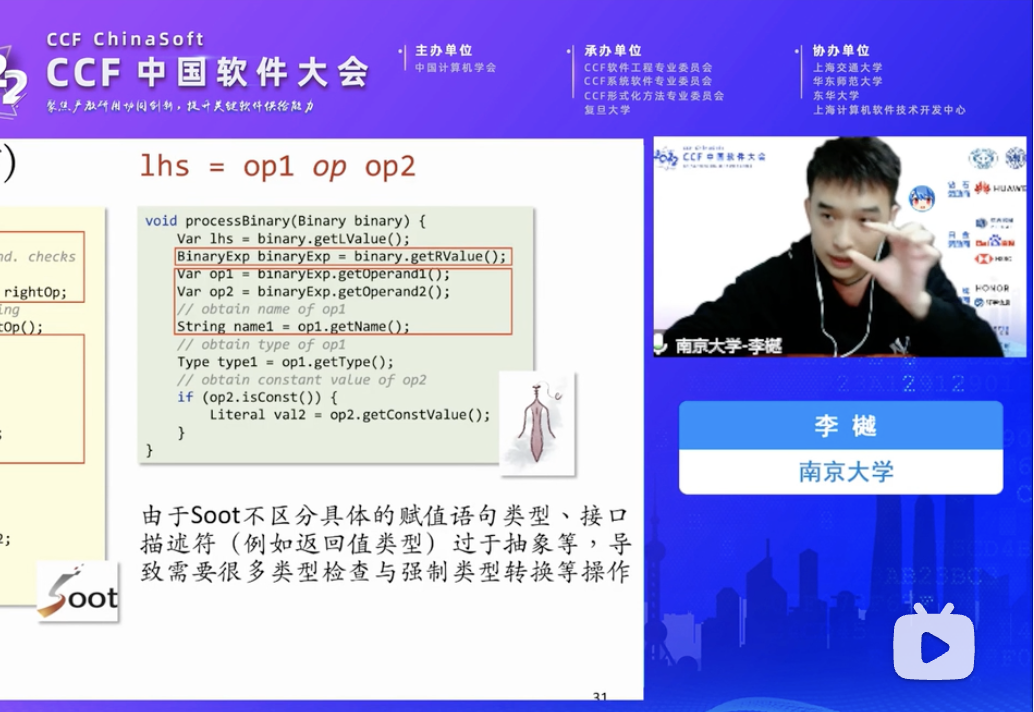
\includegraphics[scale=0.4]{1-python-plim/figs/yueli.png}
	\caption{南京大学李樾老师设计的静态程序分析框架“太阿”}
	\label{fig:ly}
	
\end{figure}

\begin{figure}[!htbp]
	\centering
	
\includegraphics[scale=0.4]{1-python-plim/figs/zihaoyu}
	\caption{余子豪的Github个人首页}
	\label{fig:yzh}
	
\end{figure}
\begin{pas}
	\begin{center}
		\large \textbf{与其说是学会提问, 倒不如说是学会不提问}
		
	\end{center}
	\begin{center}
		南京大学~蒋炎岩\\
		中国科学技术大学~余子豪(图\ref{fig:yzh})\\
		节选自《PA实验手册》
	\end{center}
	
	很多同学不多不少都会抱有这样的观点:

我向大佬请教, 大佬告诉我答案, 我就学习了.

但你是否想过, 将来你进入公司, 你的领导让你尝试一个技术方案; 或者是将来你进入学校的课题组, 你的导师让你探索一个新课题. 你可能会觉得: 到时候身边肯定有厉害的同事, 或者有师兄师姐来带我. 但实际情况是, 同事也要完成他的KPI, 师兄师姐也要做他们自己的课题, 没有人愿意被你一天到晚追着询问, 总有一天没有大佬告诉你答案, 你将要如何完成任务?

如果你觉得自己搞不定, 你很可能缺少独立解决问题的能力.

但幸运的是, 这种能力是可以训练出来的. 你身边的大佬之所以成为了大佬, 是因为他们比你更早地锻炼出独立解决问题的能力: 当你还在向他们请教一个很傻的问题的时候, 他们早就解决过无数个奇葩问题了. 事实上, 你的能力是跟你独立解决问题的投入成正比的, 大佬告诉你答案, 展示的是大佬的能力, 并不是你的能力. 所以, 要锻炼出独立解决问题的能力, 更重要的是端正自己的心态: 你来参加学习, 你就应该尽自己最大努力独立解决遇到的所有问题. 

\end{pas}


很多问题都可以通过查资料解答. 其中, 有一个很好的途径就是先看一看官方文档. 通常官方文档都有非常详细的解释. 

\begin{Exercise}\label{ex:tool3}
	如下的问题是有趣的. 它可以让你在你自己的领域当个创世神. 
	\Question 请结合给出的资料, 结合自己的思考, 写一篇《如何科学地提问》读后感, 并且在有人问出比较不适宜的问题的时候可以甩给他看, 使得他可以重新问出符合身份的问题. 
		\Question 请用Python写一段代码, 它可以模拟图灵机的行为(内存大小不是无限的, 输入输出格式自定). 
\end{Exercise}


\begin{multicols}{2}
        \begin{Answer}[ref={ex:tool3}]
			其实, 第一个问题是《一生一芯》计划中必须要有的基本素质. 倒是不如说, 越早具有这样的意识, 对自己作为计算机系的学生就越来越有益.
			
			第二个问题给出一点提示: 我们可以使用Python里面的列表来模拟一堆网格, 用变量来模拟当前值. 至于程序嘛... 输入可以采用字典的形式, 这样就可以判定自己应该往哪里移动了. 如果不行的话, 试着自己问问ChatGPT! 
			
			           	
        \end{Answer}
    \end{multicols}


\section{C语言引导}

一个很好玩的事情是, C语言程序设计的基本语法比Python更加的基础. 而且C基本代码的语义的确定的掌握要花费的精力是远远小于Python的. 它更简单、包袱更少,也没有很庞大的工具链。虽然说这相当于 “把你的手脚捆起来编程”,但我们通常不需要很复杂的数据结构和代码逻辑,因此现代语言特性的好处在大部分时候并不显著。而且用 C 语言还有一些额外的好处:

\begin{quote}
	和其他编程语言相比,C 语言特性更容易真正掌握和深入理解.如果你没有学好,用几周的时间补上应该也没问题
	C 是一种 “高级的汇编语言”, 你不难在大脑里把 C 出代码翻译成指令序列; 但对于现代语言来说, 这要困难得多. 
	透过对 C 语言的深入理解, 可以更好地理解现代编程语言的设计动机和实现方法. 
	
	 \hfill --蒋炎岩, 操作系统课程自救指南 

\end{quote}

所以, 不用惊慌. 我们会来简单介绍一下. 我们会用几个例子来说明一下C语言里面, 一些规则. 但是不用试图记忆, 最好能够跟着敲一遍. 一个比较完好的编译器会在你犯错误的时候(通常情况下犯错是很正常的)给出你提示. 这时候查一查字典就可以解决大多数的情形. 

\subsection{作为不太好用的计算器}
作为计算机, 一个很重要的事情是: 如何使用计算机进行比较复杂的算术运算? 

比如下面的程序可以告诉我们1+1的值, 并且输出到屏幕. 

\begin{lstlisting}[language=C]
#include <cstdio.h>
int main(){
	printf("%d\n", 1+1);
	return 0;
}
\end{lstlisting}

这里的``\texttt{\%d}''是输出的占位符, 会输出整数. d是digit的简称. 因为整数是由一位一位的数码构成的. 

我们来看一看有没有什么有趣的实验: 

\begin{example}
	修改程序, 输出(1) $3-4$; (2) $5\times 6$; (3) $8\div 4$; (4)$8\div 5$的值.
\end{example}

和Python不同, C会默认地把1.6转化成整数. 这是为什么? 

\begin{pas}
(Generated from ChatGPT)


	In the early days of computing, hardware resources were limited, and memory and processing power were at a premium. The ability to perform automatic conversions between different data types was therefore an important feature of programming languages, as it allowed programmers to work with limited resources more efficiently.

Additionally, the automatic conversion of float to int likely reflects the fact that early computer hardware often did not support floating-point arithmetic natively. Floating-point arithmetic was typically implemented in software, which was slower and less efficient than the native integer arithmetic. Therefore, it was often necessary to convert floating-point values to integers in order to perform arithmetic operations more efficiently.

As hardware capabilities have evolved over time, the automatic conversion of float to int in C has remained an important feature, as it provides a convenient way to work with different data types and to simplify code. However, it's still important for programmers to be aware of the potential loss of precision when converting between data types, and to use these conversions intentionally and with care.
\end{pas}

对于实数, 我们可以使用\texttt{\%f}输出. f是float的简称, 用来表示这是一个浮点数(也就是实数, 因为小数点会``浮动'').  

\begin{bonus}
	C是一个强类型的语言--也就是每一个变量都有一个一旦声明不能更改的类型. 

	如果我们输出8/5.0, 用\%f和\%d输出有什么区别? 在输出的过程中你认为的类型变换的过程如何?
\end{bonus}

如果我们在程序的开头加上\texttt{\#include <math.h>}, 就可以得到更加多样的数学运算. 如: 要计算$1+{2\sqrt 2 \over 5-0.1}$, 我们就可以在\texttt{main(){}}里面替换上

\begin{lstlisting}[language=c]
	printf("%.2f\n", 1+2*sqrt(3)/(5-0.1)); 
\end{lstlisting}


\begin{idea}
	理解代码的核心方法(上): 像阅读数学公式那样, 通过代换法理解一行代码. 
	
	举个例子, 我们在理解上面的内容的时候, 可以拆分成若干个部分, 想一想每一部分做了哪些输出. 最后整合起来就好了. 
	
\end{idea}

\subsection{变量的引入}

我们上面已经可以计算东西了, 可是还是不够劲啊! 如果我们能够从键盘读取输入就更加不错了! 那我们就需要用到\texttt{scanf}了. 

输入的东西放在哪里呢? 可以放在小盒子里面. 和Python的``小盒子''不是很相同, 小盒子必须指定变量, 并且指定了之后不能修改盒子的类型. 这也是历史上的因素导致的. 

我们来试一试: 比如最简单的$a+b$问题: 输入两个数, 用程序把它求和, 结果输出出来. 

\begin{lstlisting}[language=c]
#include <cstdio.h>
int main(){
	int a, b;
	scanf("%d%d", &a, &b);
	printf("%d\n", a+b);
	return 0;
}
\end{lstlisting} 

这时候, 代换的方法仍然起作用. 我们就可以通过交互的情况下得到输入与输出了! 

回忆一下小学的时候, 我们总是被要求计算(有点无聊的)圆柱体的表面积. 如果有一个小程序可以帮助当时的我们, 输入半径和高, 自动为我们输出答案, 那样自己就很好了. 于是我们有: 

\begin{lstlisting}[language=c]
#include <stdio.h>
#include <math.h>
int main(){
	const double pi = 3.14;
	double r, h, s1, s2, s;
	scanf("%lf%lf", &r, &h);
	s1 = pi*r*r;
	s2 = 2*pi*r*h;
	s = s1*2.0 + s2;
	printf("Area = %.3f\n", s);
	return 0;
}	
\end{lstlisting}

\subsection{顺序执行的程序}

上面我们编写了很多行的代码, 一个问题是我们的程序是怎样被执行的? 事实上, 这点和Python区别不大--在没有控制执行的情形下都是顺序--从上到下一行一行执行的. 我们可以使用调试器来证明这一点. 

\begin{tool}
	根据观察, 有很大一部分学生甚至不知道调试器是什么! 这件事情是很糟糕的--因为这样下来很多时候就会让他们看程序``一头雾水'', 然后这就是放弃的前兆. 

	所以个人认为作为一个很重要的工具--调试器在刚开始的时候就应该介绍一下. 这个工具可以帮助我们看到计算机里面到底发生了什么, 从而理解我们的输入到底在干什么. 我们可以为我们的程序打上断点(breakpoint), 然后启动调试--程序就会自动停下了, 同时把现在的状态告诉我们. 
\end{tool}


\ti{例子: 交换变量}

我一直一来是不太赞成初学的时候使用Python的语法特性\texttt{a, b = b, a}来做交换变量的. 其原因是可能会让一部分关键的直觉和感受丢失. 比如, 如果我们在C中希望交换两个变量, 怎么办? 

如果我们还想像Python那样, 看一看会得到什么: 

\begin{lstlisting}[language=c]	
$ vim tmp.c

#include <bits/stdc++.h>
int main(){
    int a = 1, b=2; 
    a, b = b, a;
    printf("a=%d, b=%d", a, b);
    return 0;
}

:!gcc %.c

warning: left operand of comma operator has no effect [-Wunused-val
ue]
    a, b = b, a;
    ^
tmp.cpp:4:15: warning: expression result unused [-Wunused-value]
    a, b = b, a;
              ^
2 warnings generated.
\end{lstlisting}

哦, 出警报了, 我们看一看运行之后会有什么效果: 

\begin{lstlisting}
:!./a.out
a=1, b=2
\end{lstlisting}

诶, 完全没有效果了! 我们回顾上面的警告说这句话没有任何的作用. 这样就解释了这件事. 所以我们要用更加底层的方法来完成. 

我们现在有哪些工具呢? (1) 创建一个带有类型的盒子; (2) 为这个盒子装/修改东西; (3) 输入, 输出; (4) 新增一行(句)代码. 


\subsection{循环结构}

我们刚刚对于所有的东西这样描述不够劲啊, 毕竟我们还是只是一个一个地完成步骤的说明. 有没有方法完成自动的重复呢? 我们可以用while循环. 

那么如果我们希望在某一个地方就不用继续循环下去了, 可以用break; 如果在某一个地方跳过下面的语句继续循环, 那么可以用continue. 

与while相仿, 我们还可以用for循环. for的语法比较像$\sum$. 同样也有break和continue. 

\subsection{方便地创建多个变量: 数组}

如果我们想要创建100个变量, 我们可以不用声明a0, a1,a2,... . 我们有可以自动给一个``空间'', 就像\texttt{int a[100];}, 这样就给我们了100个变量的int类型的空间. 如果我们想访问其中的一个(比如第14个), 我们就可以用\texttt{a[14]}来访问. 注意: 数组从0开始编号, 访问\texttt{a[100]}虽然不会有报错信息, 但是这是未定义行为. 

我们可以用重复的方法来走遍一个数组里面的所有的部分. 可以和上面的\texttt{for}很方便的对应起来. 

当然我们还可以创建多个方括号, 简称为``维度''. 比如\texttt{b[100][100}就可以让我们在一个$100\times 100$的平面上面读取数据. 比如想访问第二行(从0计数)第三列(从0计数)的就可以写成\texttt{b[2][3]} 当然, 这个维度可以是任意多个的--只要不超出内存限制就没问题. 

\begin{Exercise}\label{ex:tool4}
如下的问题是很能提升工作效率的. 你会发现, 如果你用对了工具, 那么写代码也没有那么难! 
\Question 像上次一样, 自己配置好写一段C的代码的环境, 以方便自己未来调试代码的工作. 注意, 这个就不太好办了. 在你感到迷茫的时候, 可以搜索一下命令行相关的内容, 理解你的源代码是如何编译的.

\Question 找来一本《Unix传奇: 历史与回忆》 读读看! 看看当时他们是如何富有创造性地构建起来我们今天运用的一切的! 
\end{Exercise}

\begin{multicols}{2}
        \begin{Answer}[ref={ex:tool4}]
			你可以安装gcc并且使用gdb调试. 我不是很推荐直接上Visual Studio -- 太笨重, 对于初学者很不友好. 但是Visual Studio Code是很好的工具. 祝你顺利! 
			
			Unix传奇中的人都为计算机系统的发展做出了很多的贡献! 看看他们的敏锐的直觉, 感受一下穿越五十余年, 传来的那个时代的欣喜与调皮. 
        \end{Answer}
    \end{multicols}

\vspace{2cm}

\begin{quote}
	这证明了一个普遍规则:程序帮你写的代码会比你自己手写的更正 确、更可靠。如果改进了生成器,例如能生成更好的代码,那么每个人 都会受益;相反,对手写程序的改进并不能改善其他程序。像Yacc和
Lex这样的工具是这一规则的极好例子,Unix也提供了许多其他工具。 编写程序的程序总是值得尝试。就像道格·麦基尔罗伊所言,“任何你必 须重复做的事都有待自动化。”
\hfill -- Unix传奇: 历史与回忆
\end{quote}



